\chapter{MVC and HMVC design patterns}

\label{kap:courses} % id kapitoly pre prikaz ref

\paragraph{}
For software to be usefult, it has to interact with something. This could be another computer or process, or the interaction could be with people. So, there are interfaces. In modern applications, more effort often goes into development of usable interface than in other tasks. On the other side, our software needs to acces and store its data and perform operations on them. Purpose of this chapter is, at first, to explain MVC design patter, which is a simple and widespread way for solving this problem, then we will focus on extension of this pattern, HMVC. Both patterns are crucial to understand for purposes of this work.

\section{Model-View-Controller}
\paragraph{}
In an Object oriented programming (OOP) programmers often run into problems with application complexity and maintanance of code. As application becomes larger and more robust, it is ofter harder to add or modify existing features. Modifying of complex classes and unclear implementation can cause a lot of software bugs. On the other way, design patterns aim to provide reusable soulutions of common problems in software engineering and reduce this complexity by splitting functionality into specific classes with a single purpose. One of the most important desing patterns is Model View-Controller, which is the performs as the core of the CodeIgniter framework, which we will discuss later.

\paragraph{}
Model-View-Controller (MVC) design pattern was first created in 70’s by SmallTalk programmers. Since that time, MVC design idiom has become a commonplace, especially in object oriented systems \cite{deacon2009model}. Motto of this pattern is specified as to "Stop data, program logic and presentation layers being mixed up together".

\paragraph{}
To do so, MVC has to split application functionality into three layers: models, views and controllers. Each part plays specific, distinctive, non-overlapping function. This also enables programmers to easily replace these layers and extend functionality. Now, let's look at each layer.

\begin{figure}[t]
    \centering
    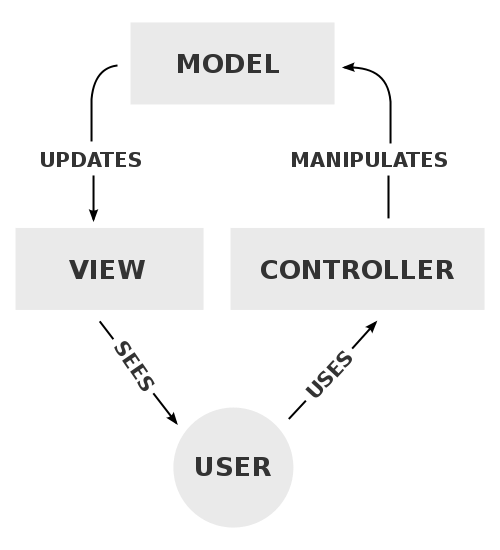
\includegraphics[width=0.5\textwidth]{images/mvc.png}
    \caption{Model-View-Controller}
    \label{fig:mvc}
\end{figure}

\subsection{Model}
\paragraph{}
The model is where all the business logic of an application is kept \cite{phpmvc}. This can mean anything from usage of third-party services via APIs to database access in order to fulfill applications business requirements. If applications needs to read or write any data, all the operations must be performed in this layer. For purposes of this work, models will mostly contain CRUD (Create-Read-Update-Write) operations with Courses database tables in PosgreSQL.

\subsection{View}
\paragraph{}
The view, as opposed to model, is where all of the user interface elements are kept \cite{phpmvc}. Very important rule is that models are just templates without any logic whatsoever. For purposes of our work, views will be only PHP templates, which directly generates HTML, CSS and JavaScript responses.

\subsection{Controller}
\paragraph{}
And finally, the controller is the component that connects models and views together \cite{phpmvc}. Over-simplifying a bit, controller knows all the enviroment settings (operating system, display resolution, ...) and according to these loads data from models, performs operations with them and then the results are sent to a view. Controller knows the views but views does not. The same applies to models.

\section{HMVC design pattern}
\paragraph{}
Using MVC design pattern is excellent for building small applications. Hovewer, huge application building on pure MVC pattern brings also some disadvantages \cite{culik}. For example, large sets of views, models and controllers could be a point of confusion and failure for many programmers. In case of larger projects, it is very needed to bring order to MVC. Solution to this problem can be Hierarchical Model-View-Controller design pattern (HMVC) \cite{hmvc}.

\paragraph{}
Hierarchical Model-View-Controller design pattern (HMVC) is a direct extension of the MVC pattern that aims to solve mainly scalability issues mensioned earlier. HMVC was first described in a blog post entitled HMVC: The layered pattern for developing strong client tiers on the JavaWorld web site in July 2000 \cite{hmvc}. In summary, HMVC is a collection of MVC triads operating as one application. Each of this triads is treated as individual and can be rendered on it's own. This resolves into greater scalability, code reusability and most importantly, resolves the problem with hudge views in large projects.

\paragraph{}
To successfuly implement HMVC, it is crucial for application to be broken into systems \cite{hmvc}. Each system gets it's own views, models and controllers and is fully in control of it's own part and nothing else. In Courses 2 system, these systems are called modules, which we will discuss later. One of the advantages of using HMVC design pattern is, that we can focus on one module without changing implementation in others.

\paragraph{}
As understanding of design patterns is needed but not considered main focus of this work, we leave any further explanations to Jakub Culik's work \cite{culik}.
